\documentclass{article}

% Set the margins of the page.
\usepackage[a4paper, total={6.5in, 9in}]{geometry}

% A bunch of math packages.
\usepackage{amssymb}
\usepackage{amsmath}
\usepackage{amsthm}
\usepackage{amsfonts}
\usepackage{mathtools}
\usepackage{float}
\usepackage[labelformat=empty ]{caption} %remove figure:# from captions

\usepackage{changepage}
\usepackage{graphicx} 		% Insert images
\usepackage{color}				% COLORS!
\usepackage[shortlabels]{enumitem}			% More enumerate types such as \alph*
\usepackage{listings}			% Used for code-blocks in latex.
\usepackage{hyperref}
% Create links when using ref and table of contents.
\hypersetup{colorlinks=true, linkcolor=black}

% Replace the indents for paragraphs with empty lines.
\usepackage[parfill]{parskip}

\usepackage[myheadings]{fancyhdr}
\usepackage{titleref}
\makeatletter
\newcommand*{\currentname}{\TR@currentTitle}
\makeatother

% Number equations with reference to sub sections.
\numberwithin{equation}{subsection}

\definecolor{lightgray}{RGB}{200, 200, 200}

% Set some style rules for code-blocks
\lstset{
	literate={<-}{$\leftarrow$}{2} {\\infty}{$\infty$}{1},
	backgroundcolor=\color{lightgray}
,
	framexleftmargin=2pt,
	framexrightmargin=2pt,
	framextopmargin=2pt,
	framexbottommargin=2pt,
	frame=single,
	basicstyle=\fontsize{10pt}{15pt}\selectfont,
	stepnumber=1,
	tabsize=4,
}


%increases table padding
\def\arraystretch{1.5}



\title{\textbf{CSCI-2201\\Lab 6}}
\author{Anas Alhadi\\B00895875}


\begin{document}

	\maketitle
	\tableofcontents


	\newpage
	\section{Exercise 1}
	\begin{center}
	\begin{figure}[H]
		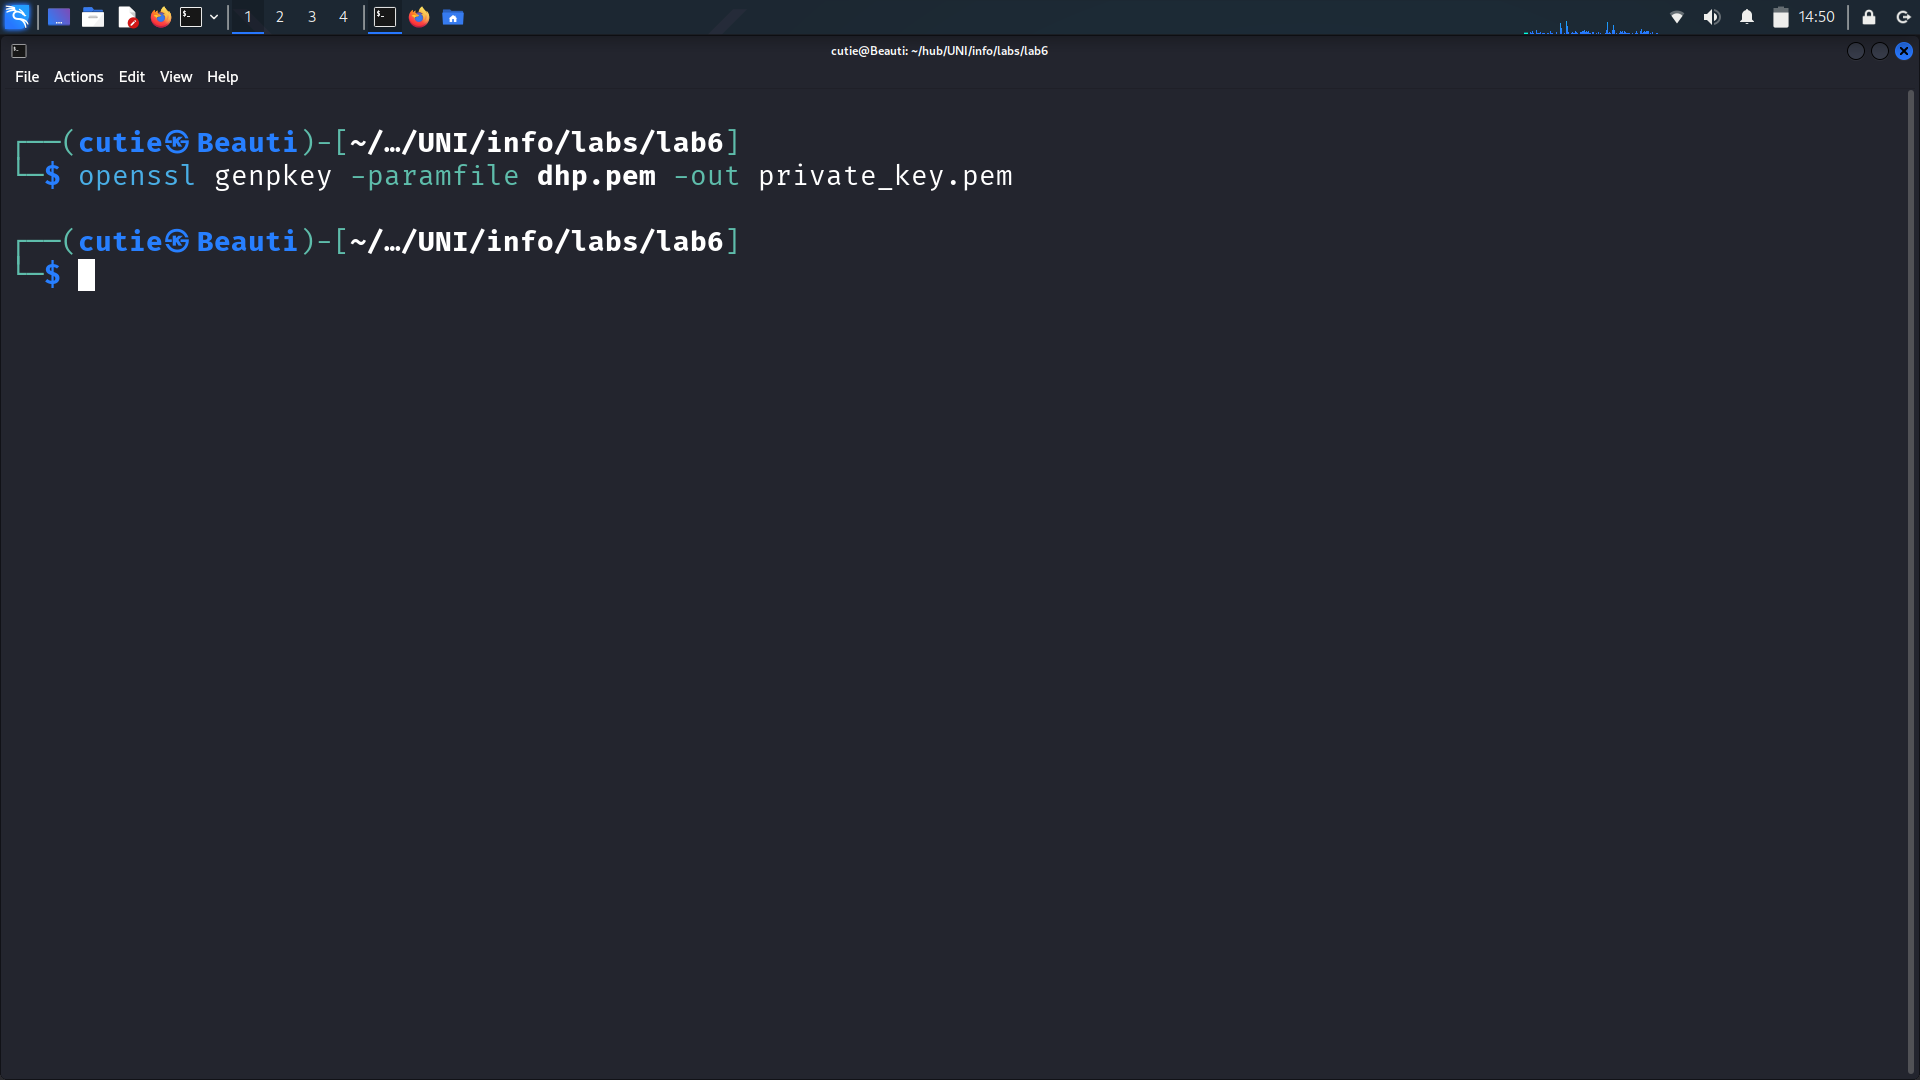
\includegraphics[width=400pt]{pic/1.1.png}
		\caption{step 1}
	\end{figure}

	\begin{figure}[H]
		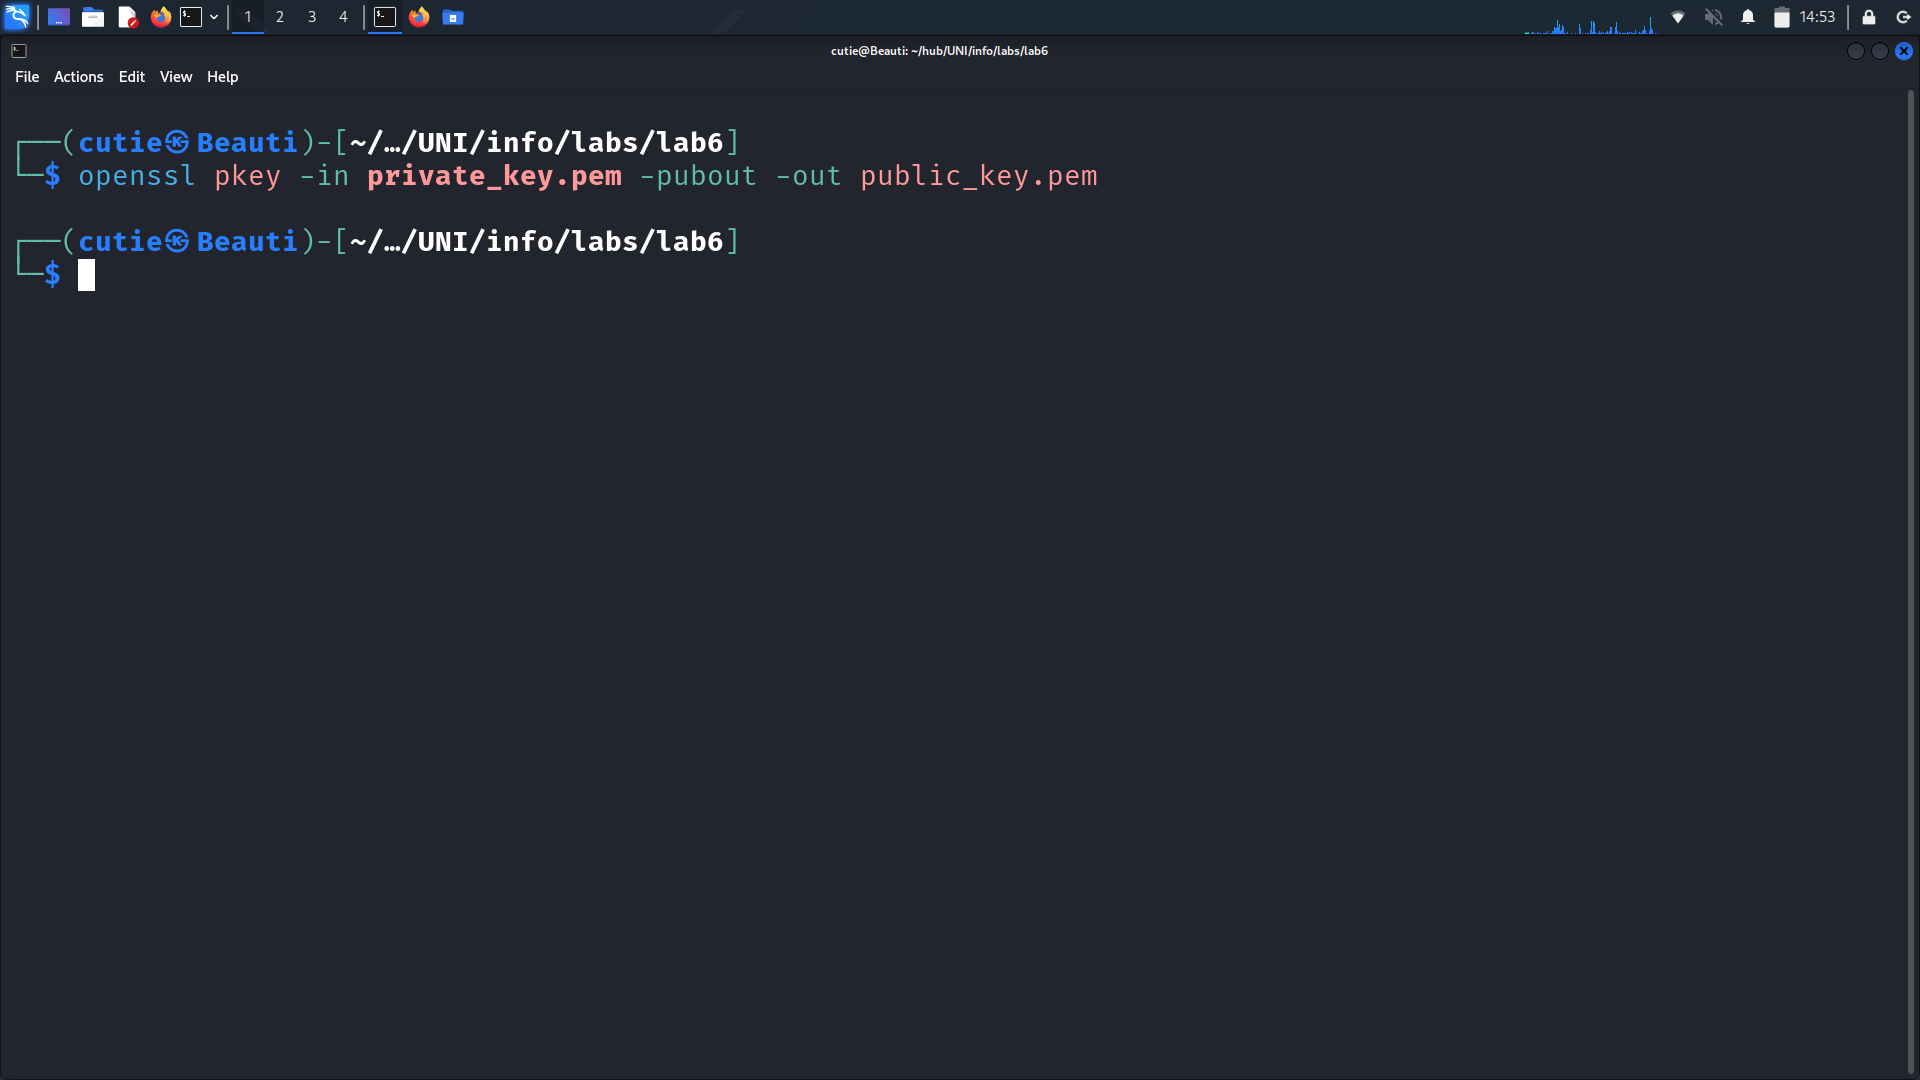
\includegraphics[width=400pt]{pic/1.2.png}
		\caption{step 2}
	\end{figure}

	\begin{figure}[H]
		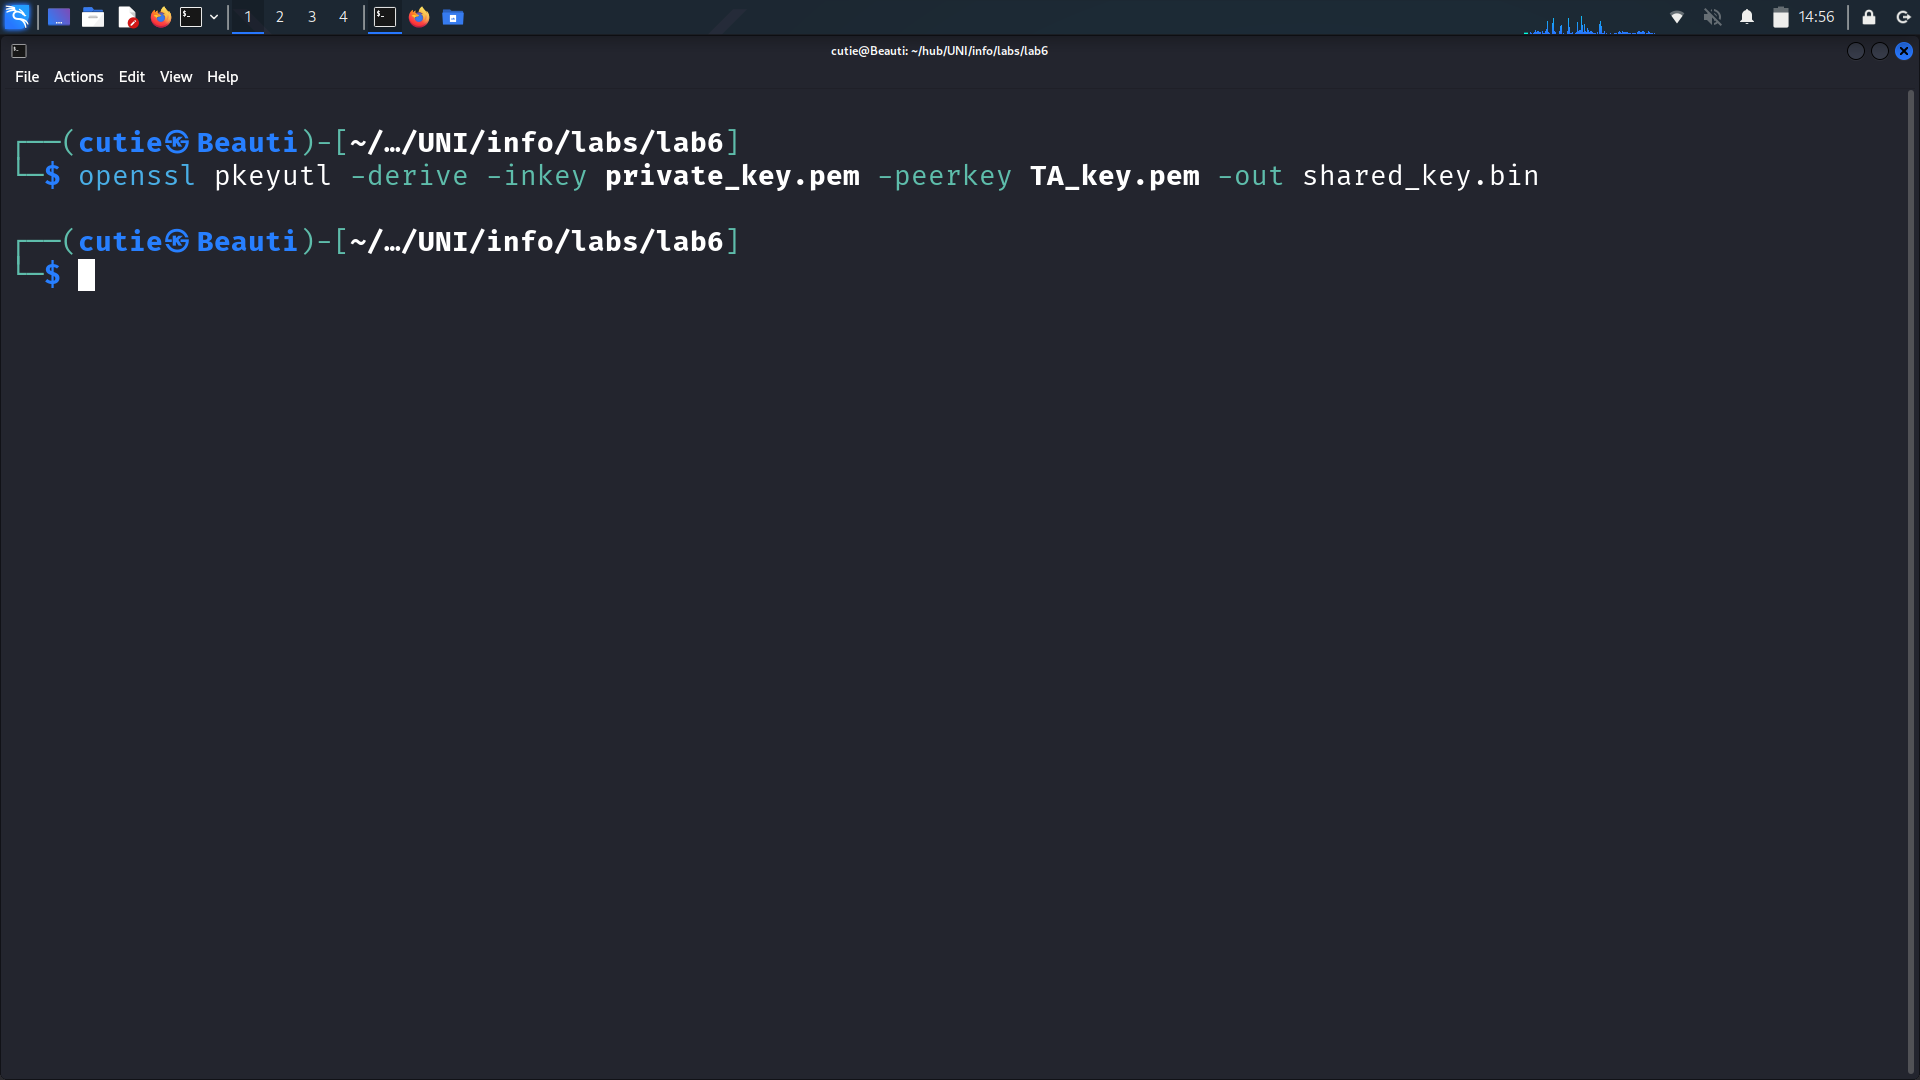
\includegraphics[width=400pt]{pic/1.3.png}
		\caption{step 3}
	\end{figure}

	\begin{figure}[H]
		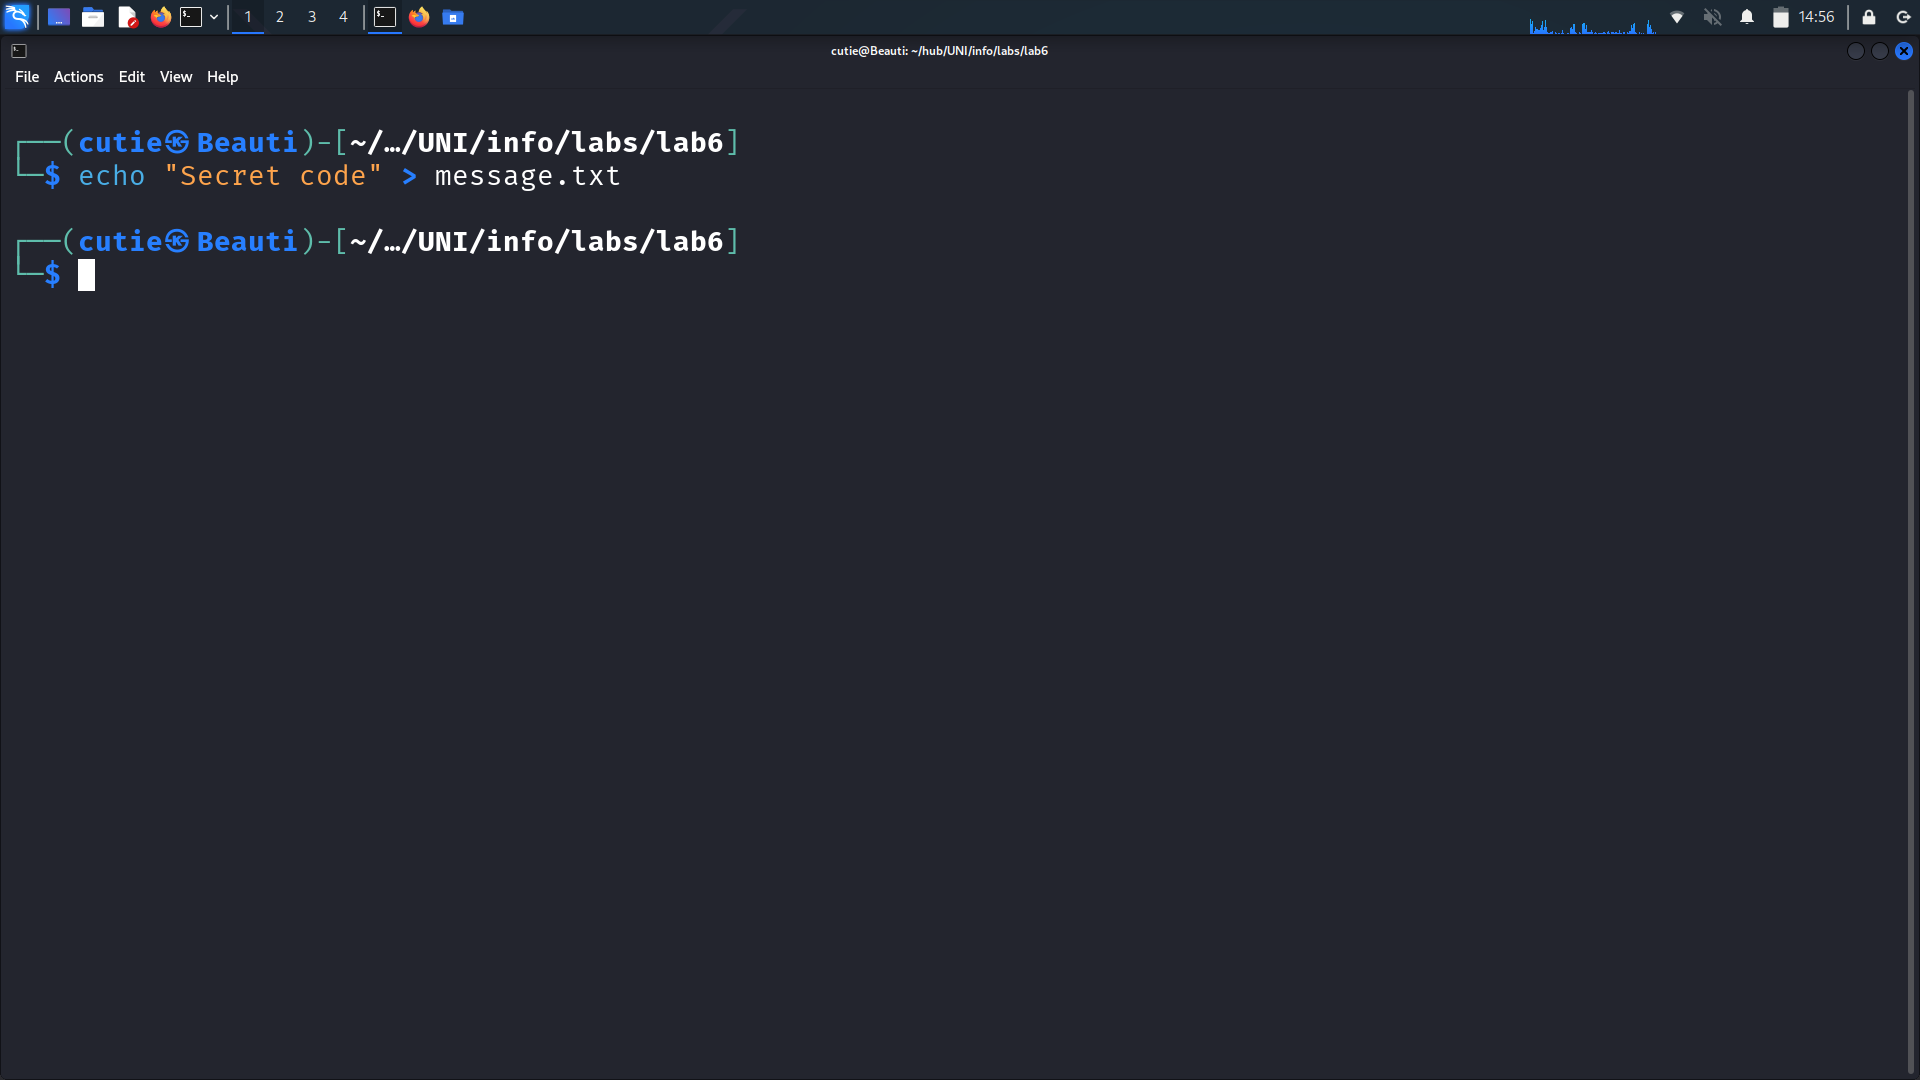
\includegraphics[width=400pt]{pic/1.4.png}
		\caption{step 4}
	\end{figure}


	\begin{figure}[H]
		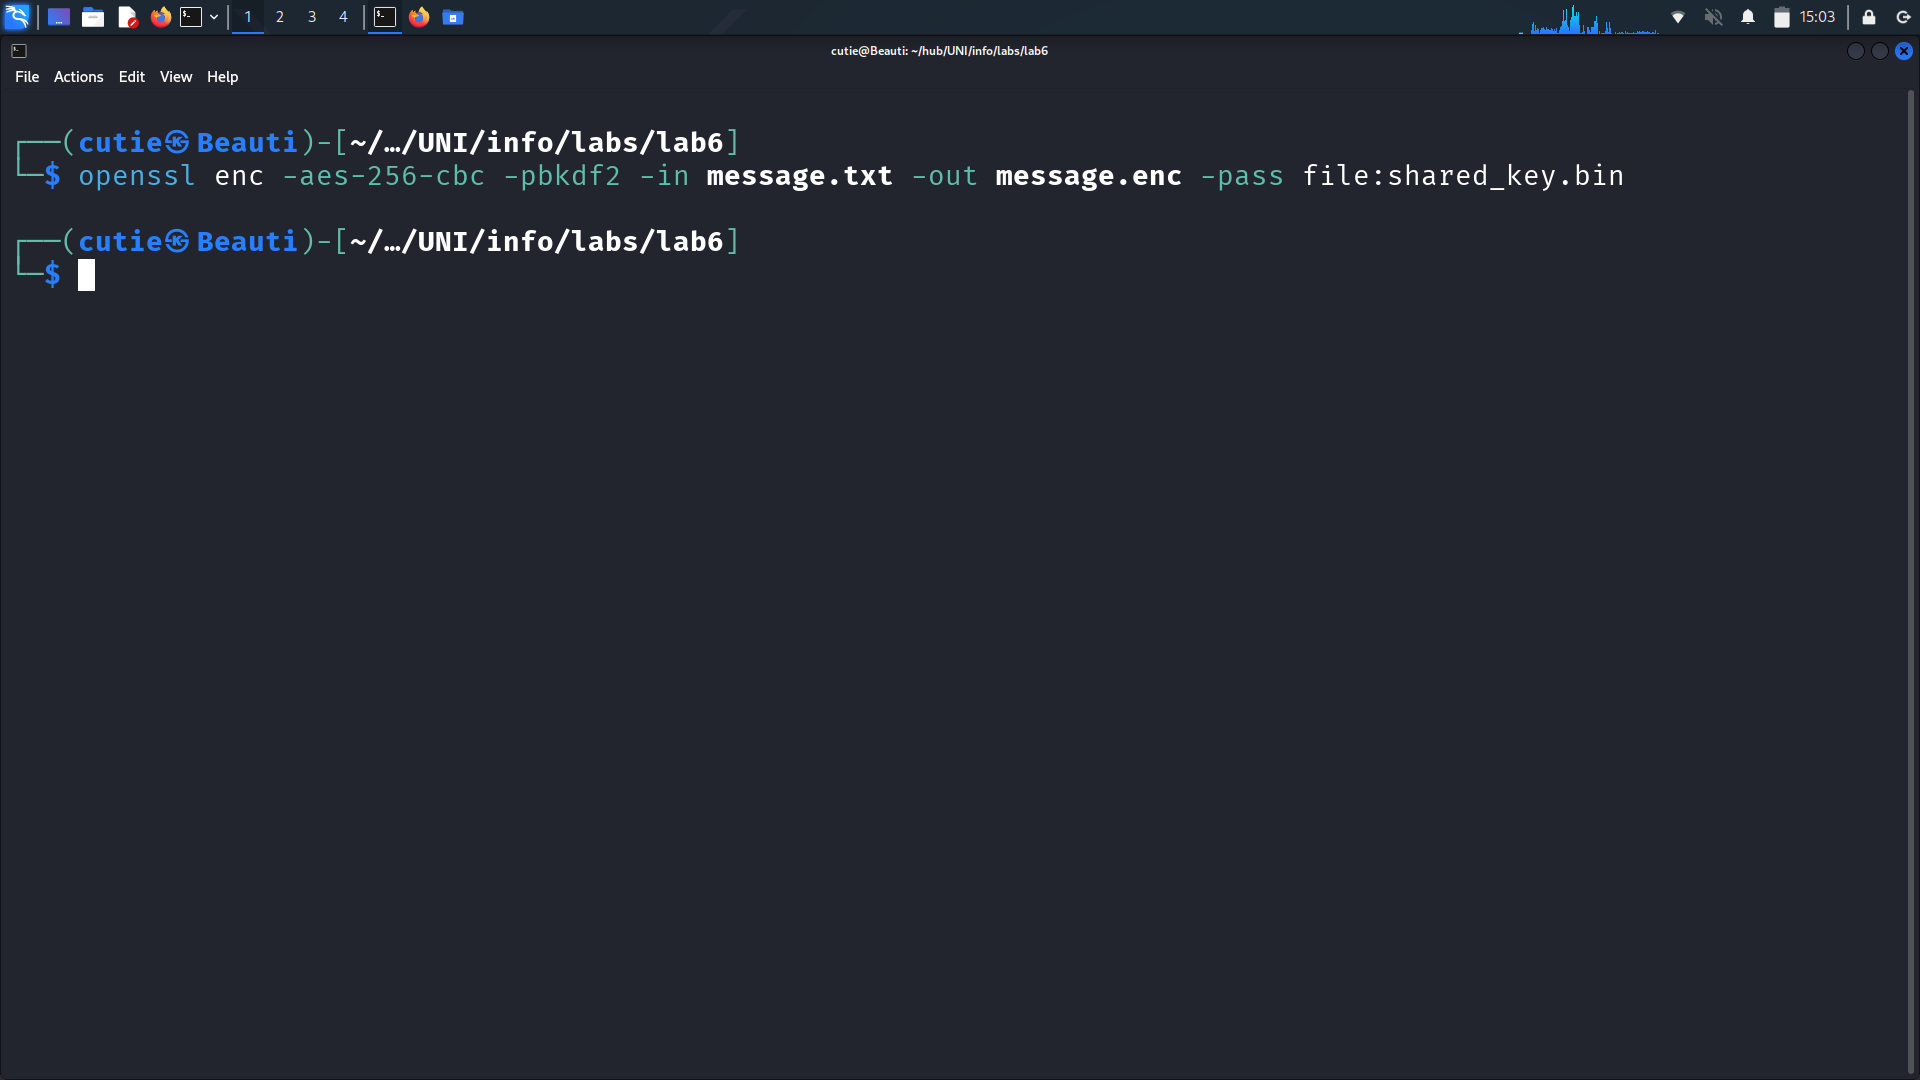
\includegraphics[width=400pt]{pic/1.5.png}
		\caption{step 5}
	\end{figure}


	\begin{figure}[H]
		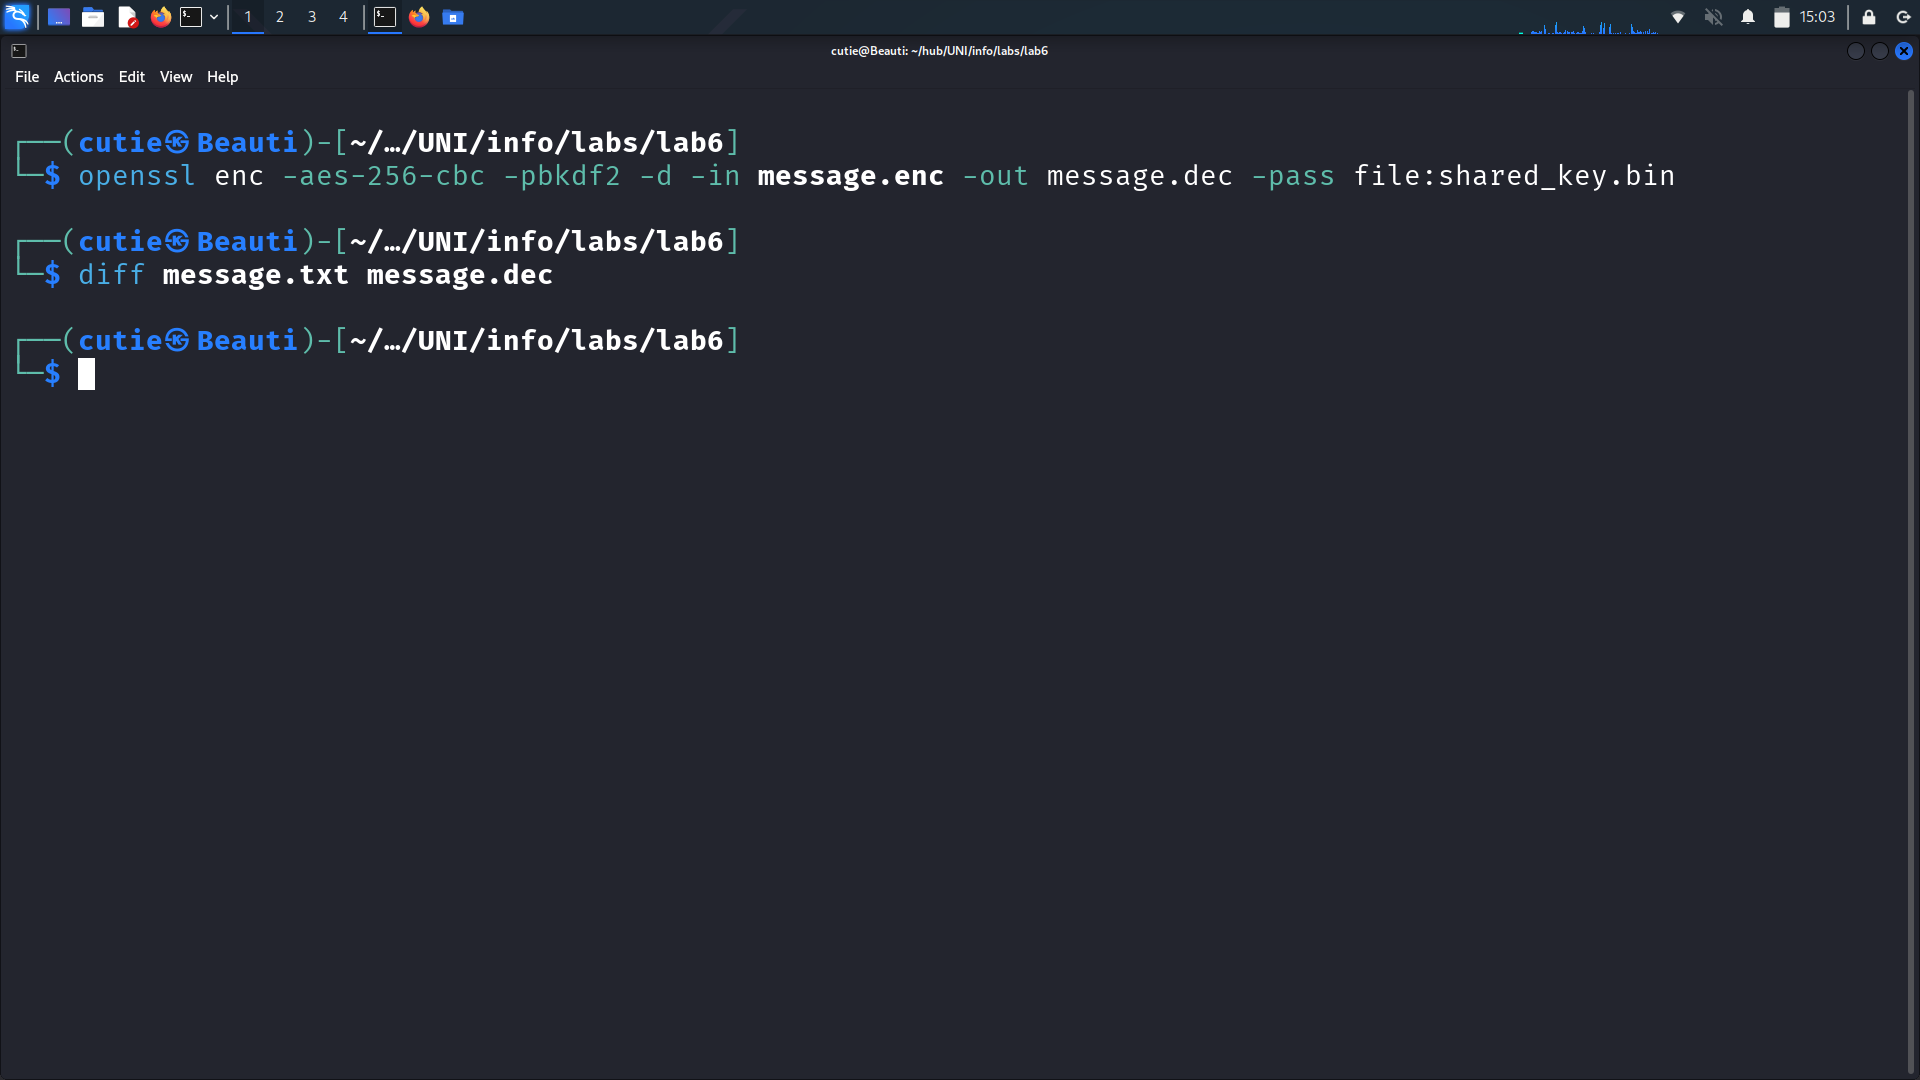
\includegraphics[width=400pt]{pic/1.6.png}
		\caption{step 6}
	\end{figure}

\end{center}

	\newpage
	\section{Exercise 2}
	\begin{center}
	\begin{figure}[H]
		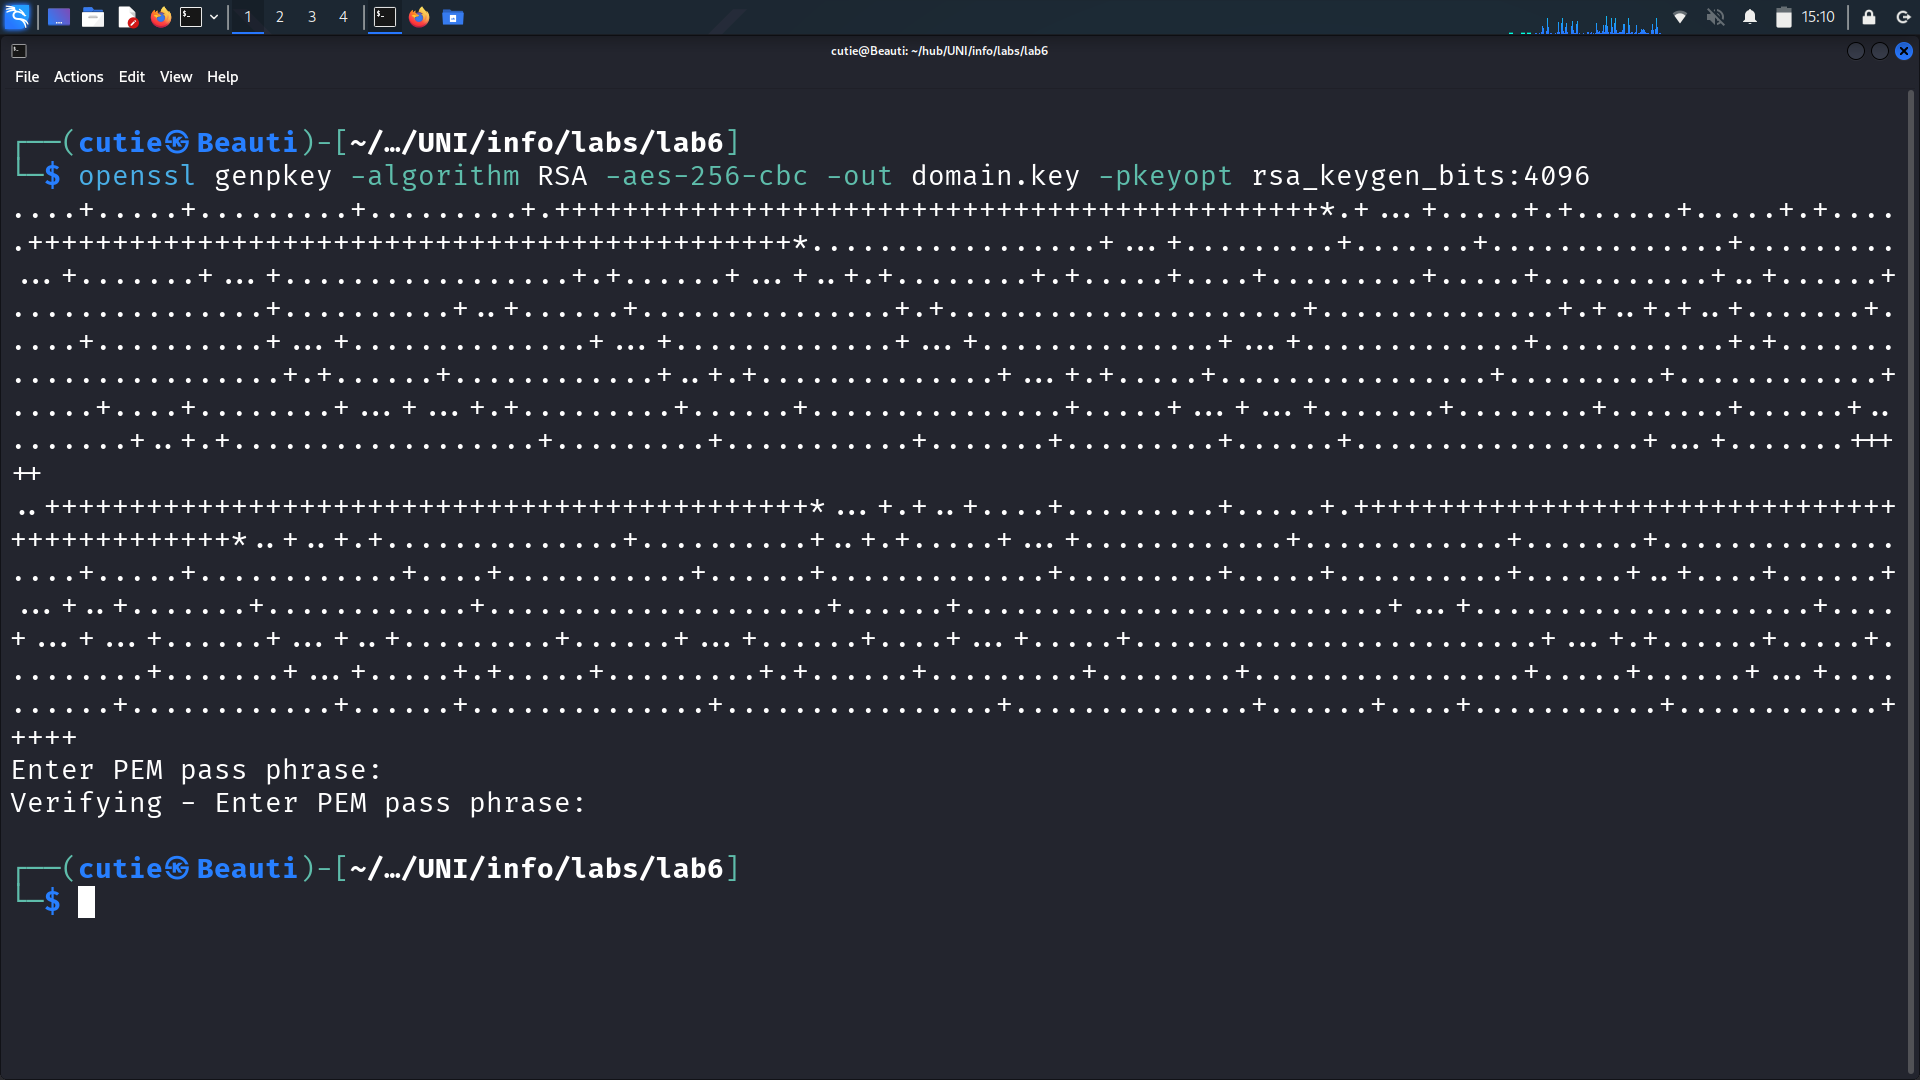
\includegraphics[width=400pt]{pic/2.1.png}
		\caption{step 1}
	\end{figure}

	\begin{figure}[H]
		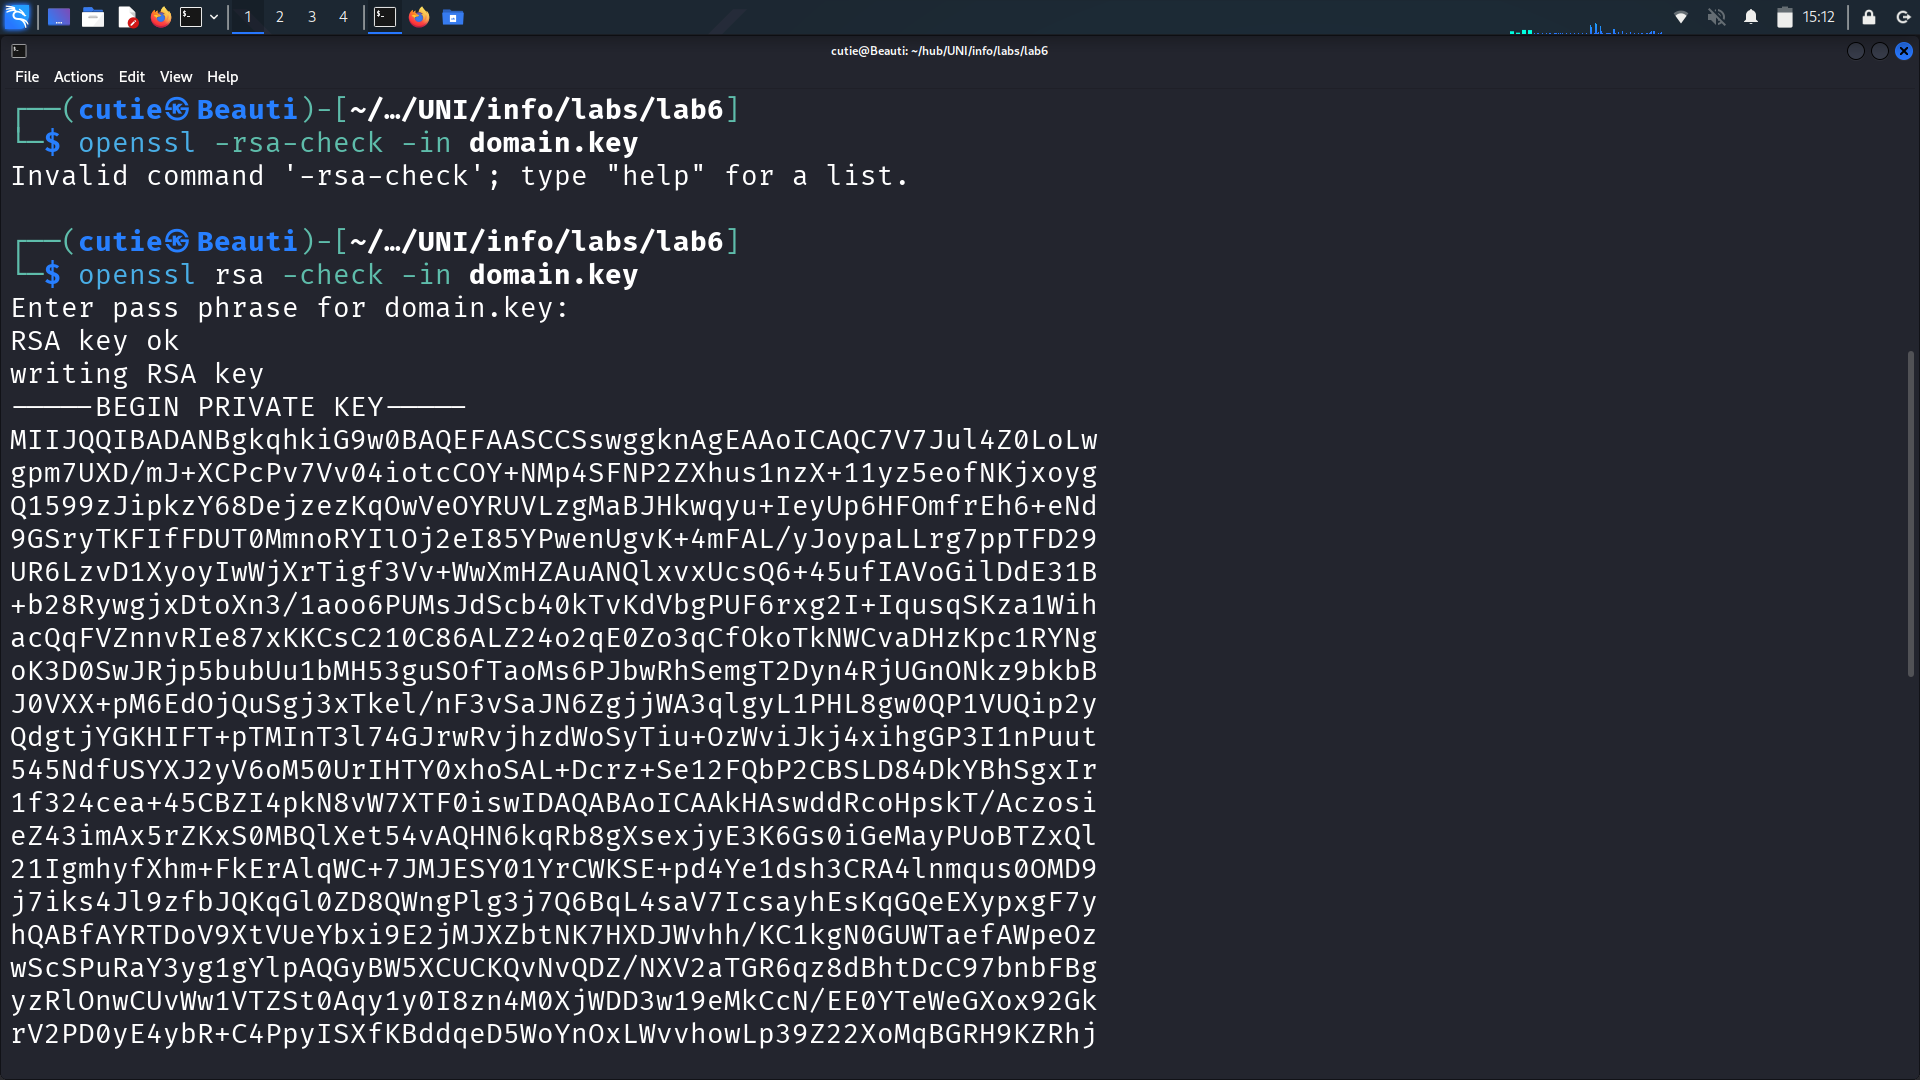
\includegraphics[width=400pt]{pic/2.1_check.png}
		\caption{checking step1}
	\end{figure}


	\begin{figure}[H]
		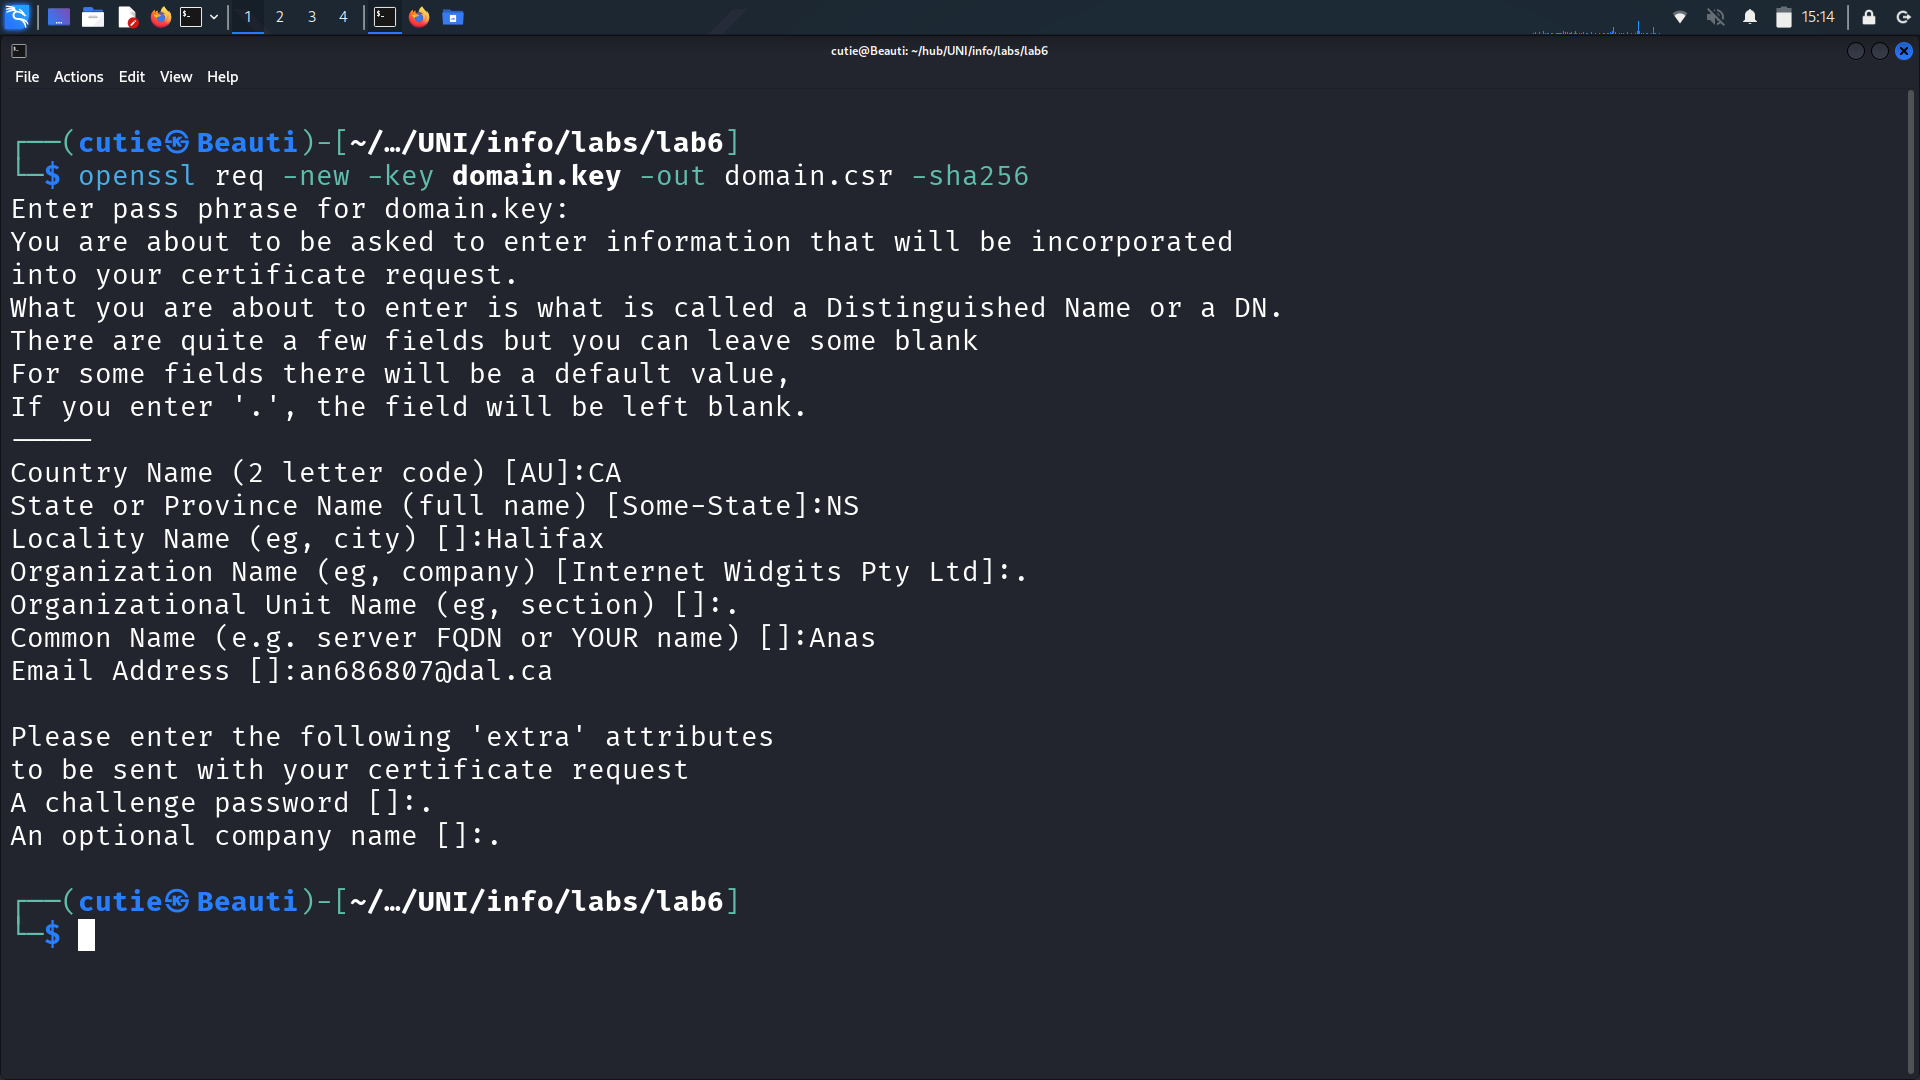
\includegraphics[width=400pt]{pic/2.2.png}
		\caption{step 2}
	\end{figure}

	\begin{figure}[H]
		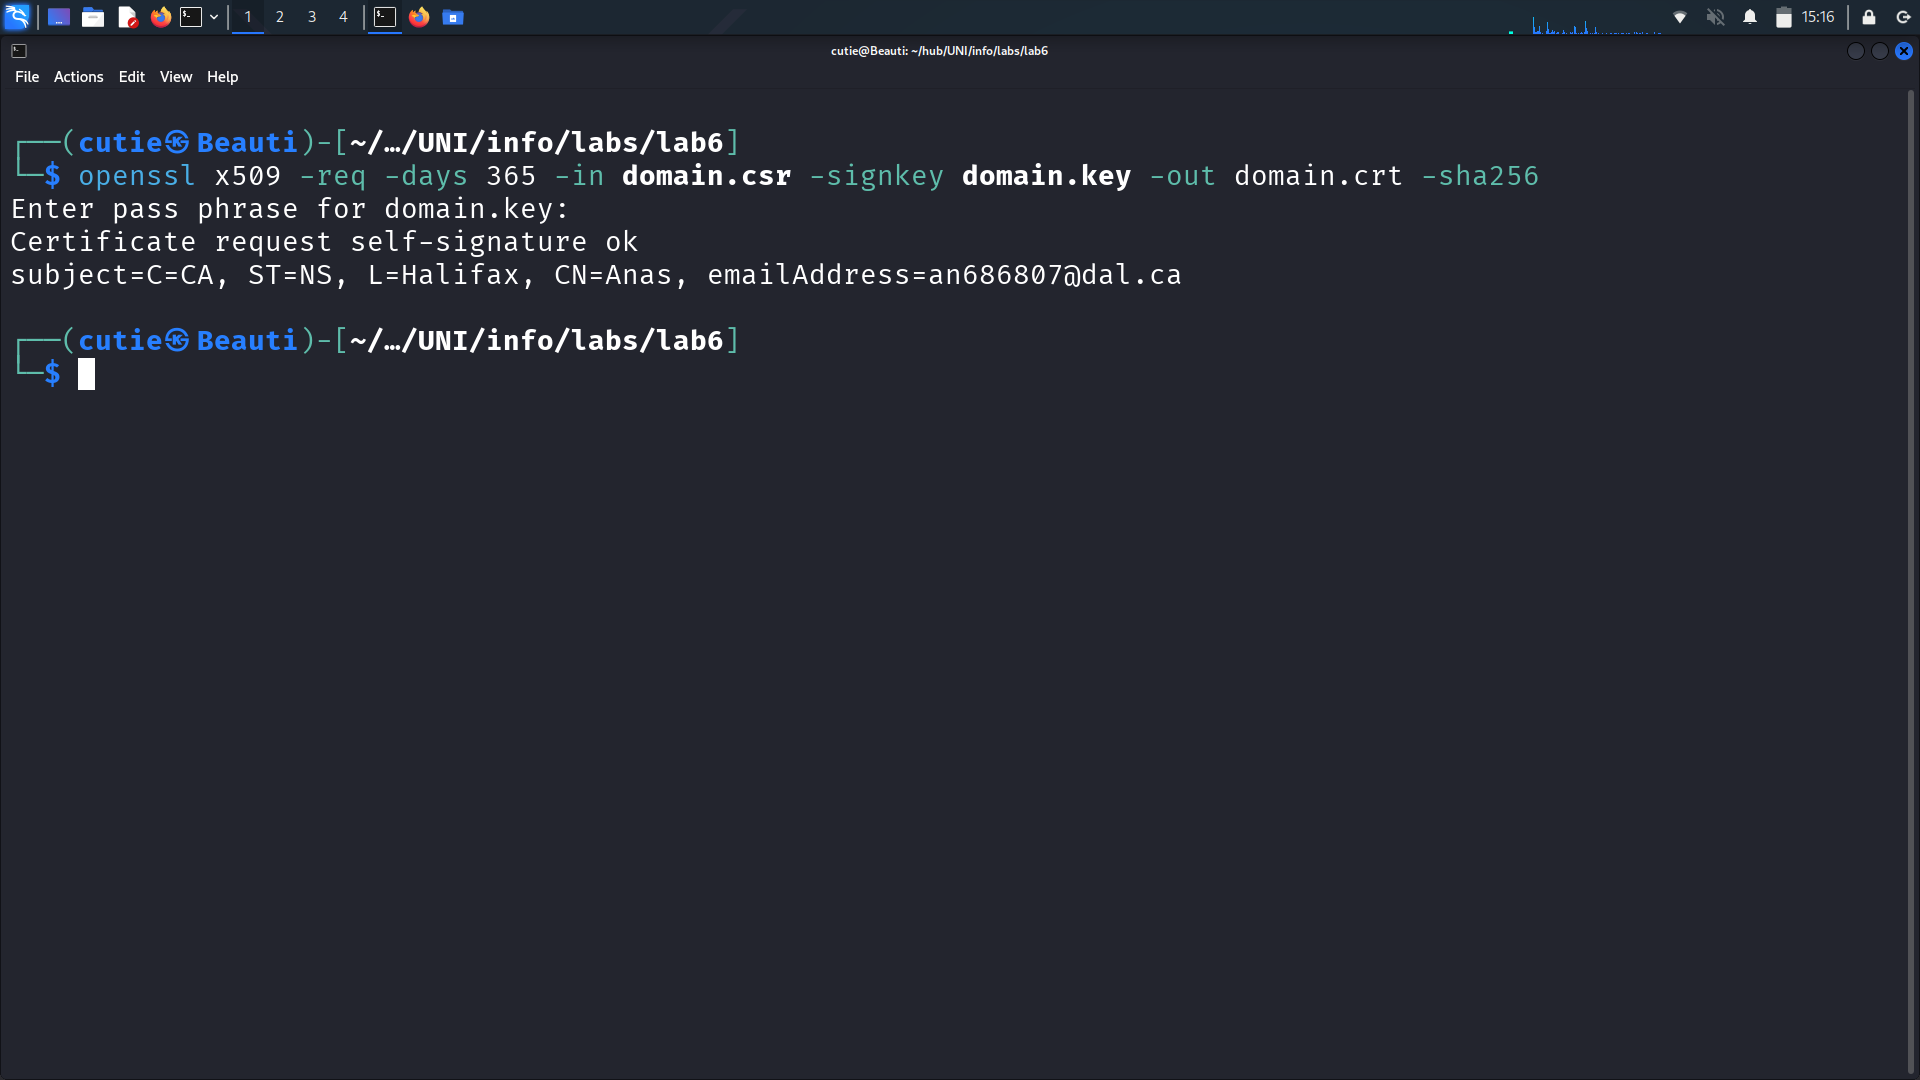
\includegraphics[width=400pt]{pic/2.3.png}
		\caption{step 3}
	\end{figure}


	\begin{figure}[H]
		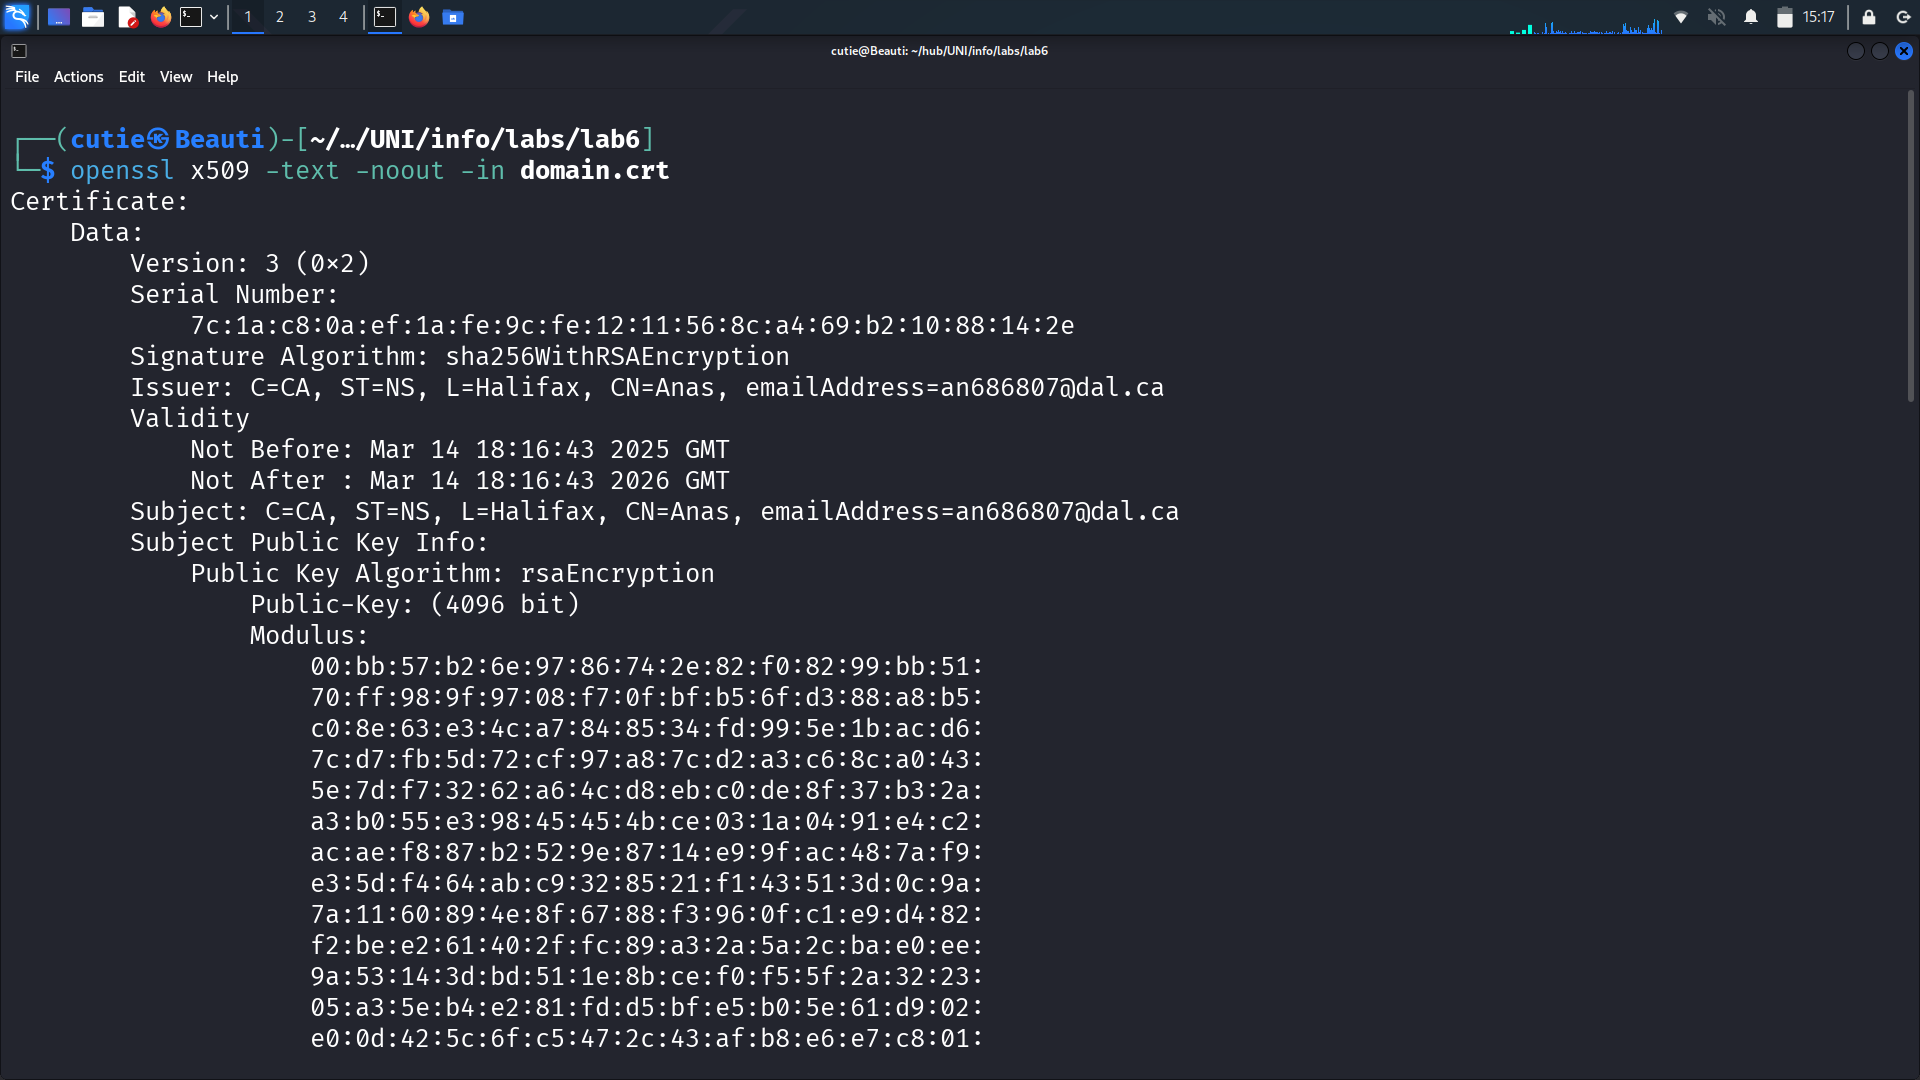
\includegraphics[width=400pt]{pic/2.4.png}
		\caption{step 4}
	\end{figure}
	\end{center}
	\newpage
	\section{Exercise 3}
	
	\begin{center}
	
		\begin{figure}[H]
		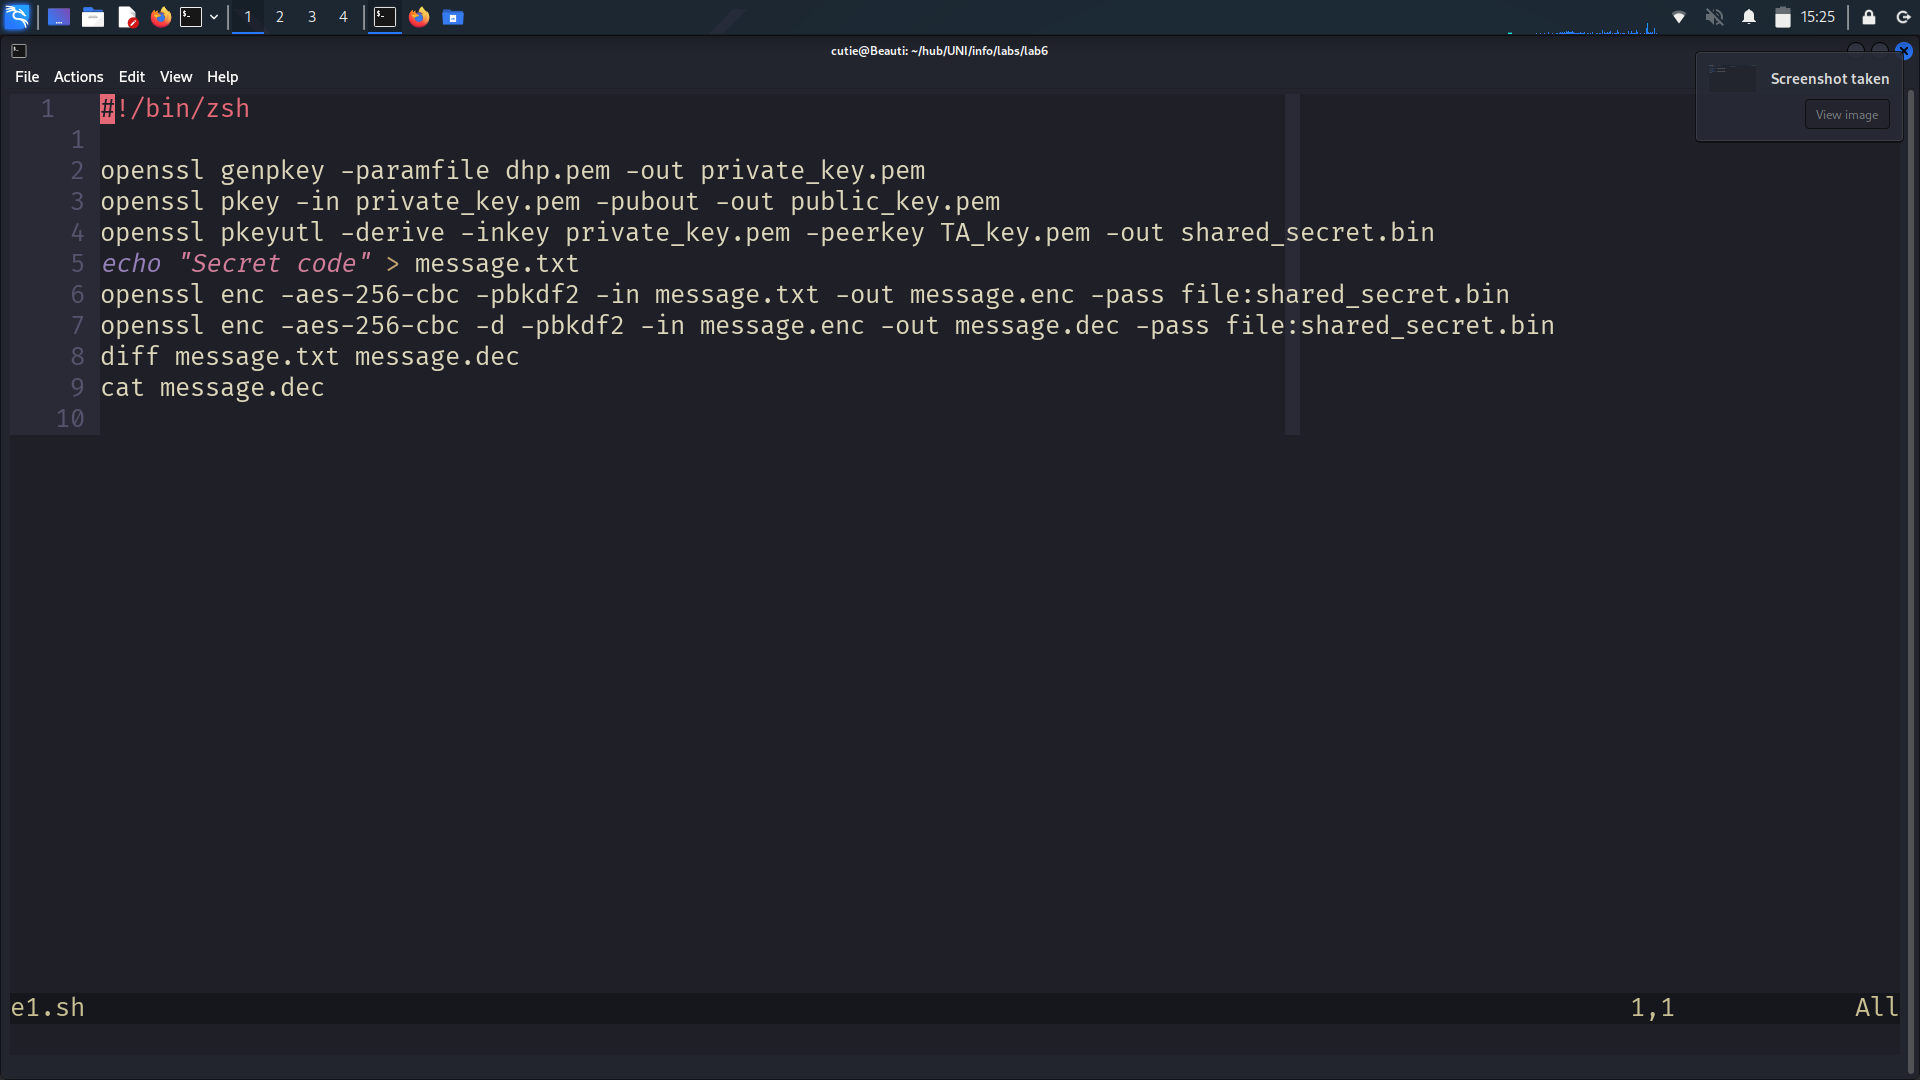
\includegraphics[width=400pt]{pic/e1_script.png}
		\caption{Exercise 1 script}
	\end{figure}

	\begin{figure}[H]
		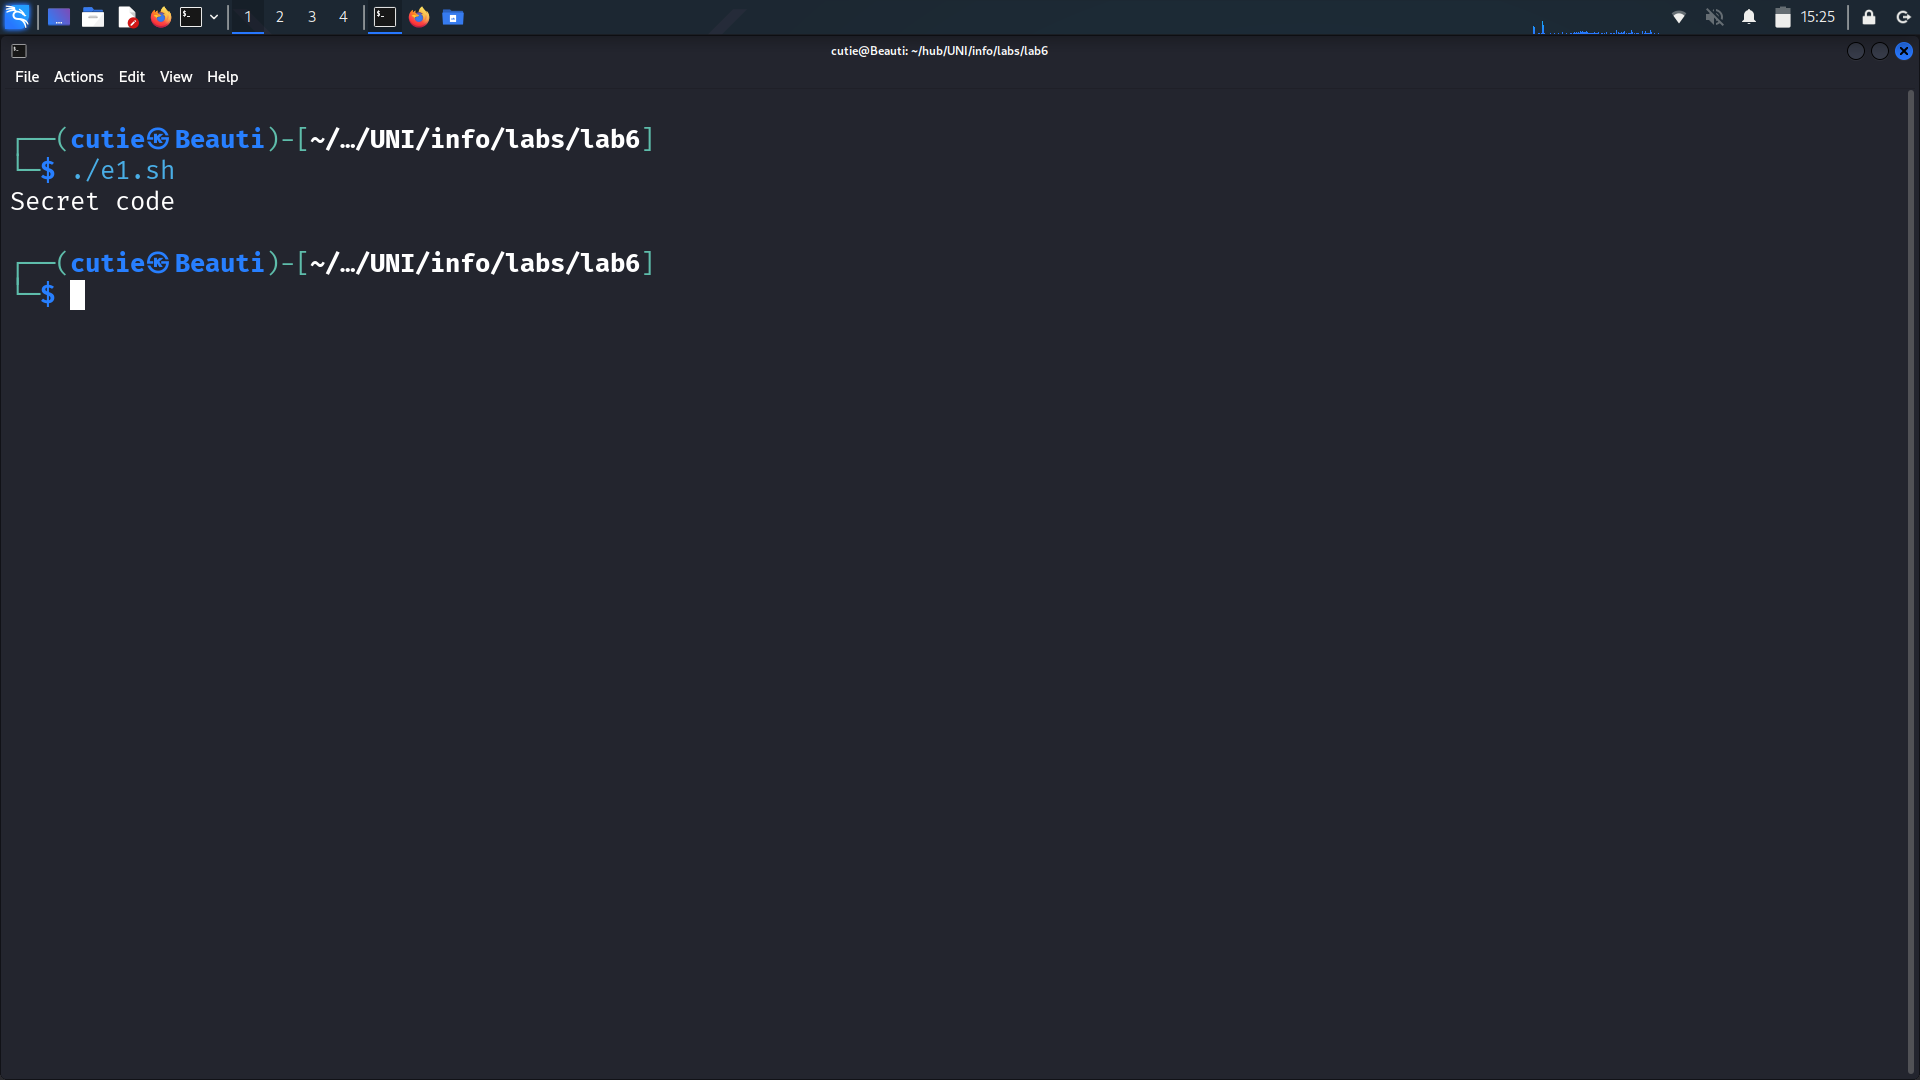
\includegraphics[width=400pt]{pic/e2_script.png}
		\caption{script check}
	\end{figure}

	\begin{figure}[H]
		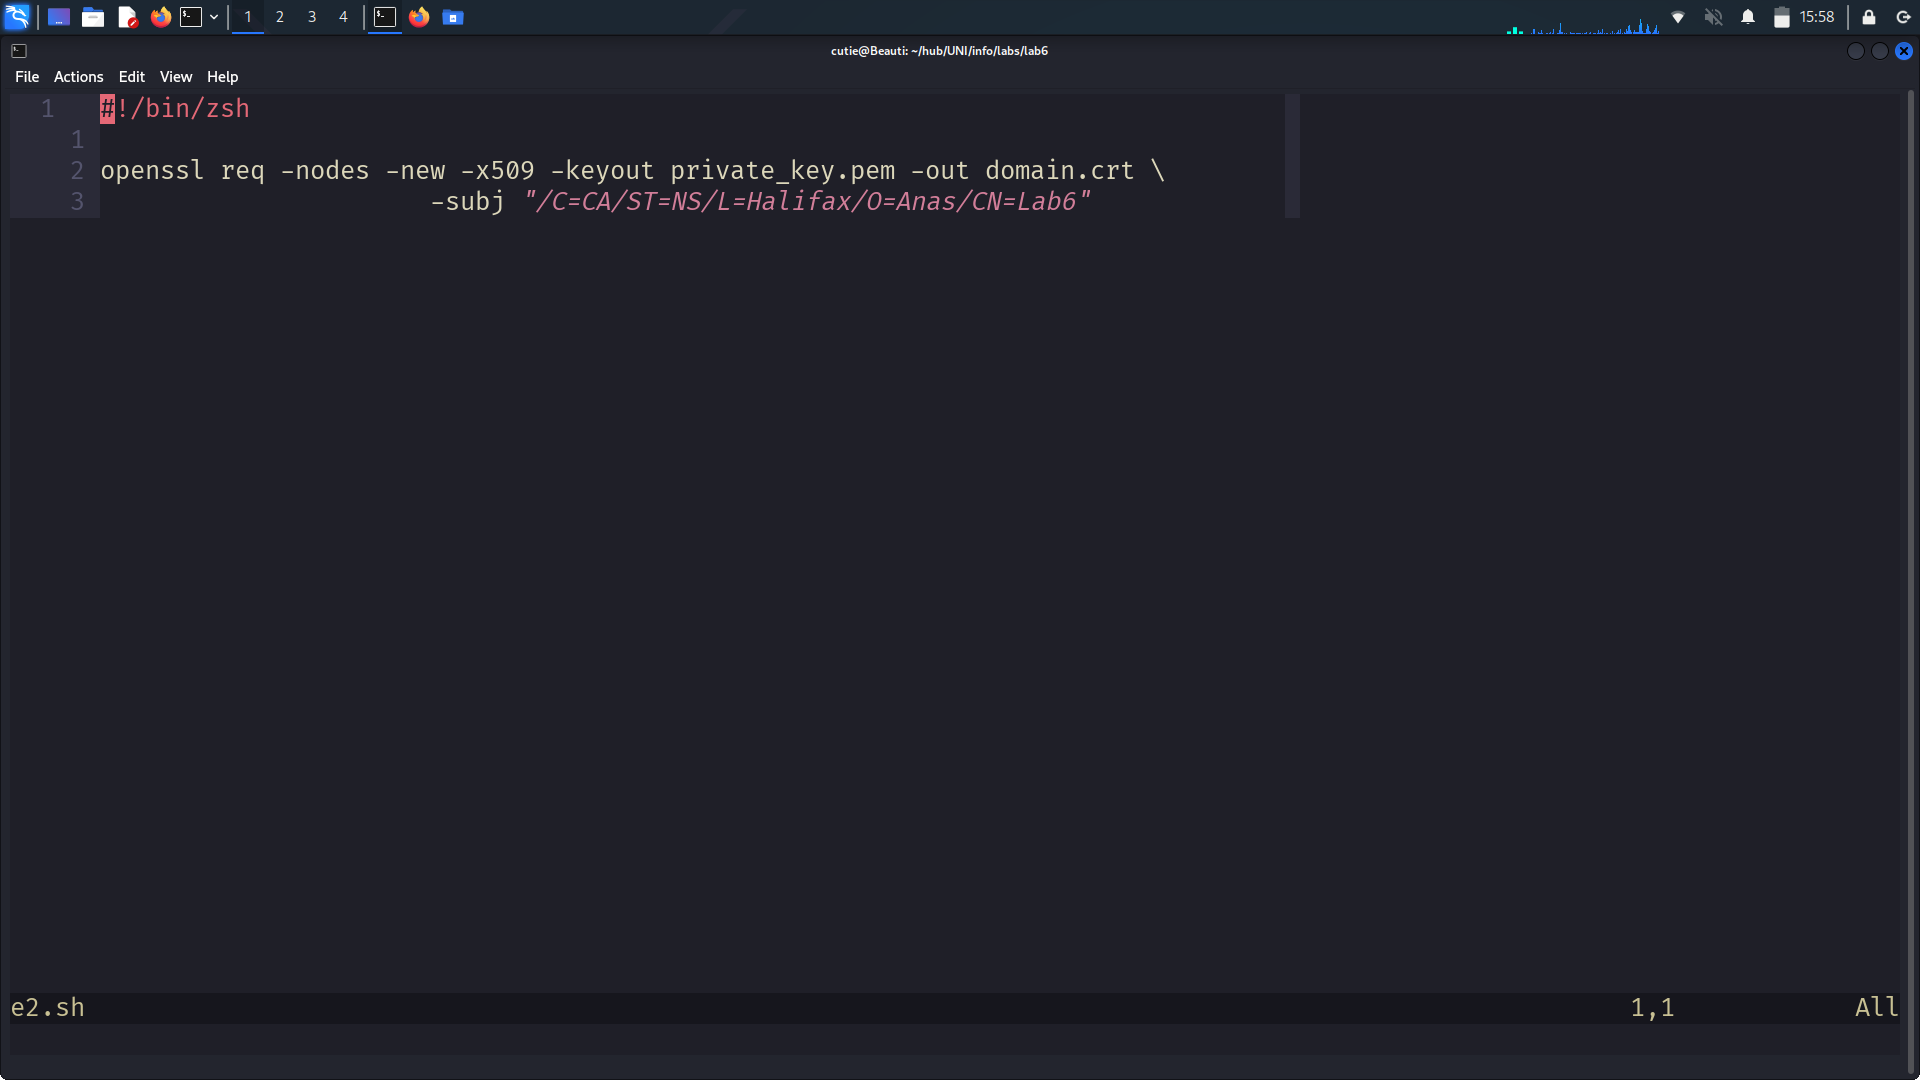
\includegraphics[width=400pt]{pic/Screenshot_2025-03-14_15_58_43.png}
		\caption{Exercise 2 script}
	\end{figure}

\end{center}

	\subsection{Algorithms:}
	We can use the command ``openssl ciphers -v" to list all of the available algorithms, some
	that I have access to are:
	\begin{enumerate}
		\item AES(256) 
		\item AESCCM8(256)
		\item Camellia(256)
		\item SEED(128)
		\item CHACHA20/POLY1305(256)
	\end{enumerate}
\end{document}
